\vspace{10pt}

{\centering\subsection*{龙紫怡:我的乐园}}

\addcontentsline{toc}{subsection}{龙紫怡:我的乐园}

\renewcommand{\leftmark}{龙紫怡:我的乐园}

\begin{figure}[htbp]

\centering

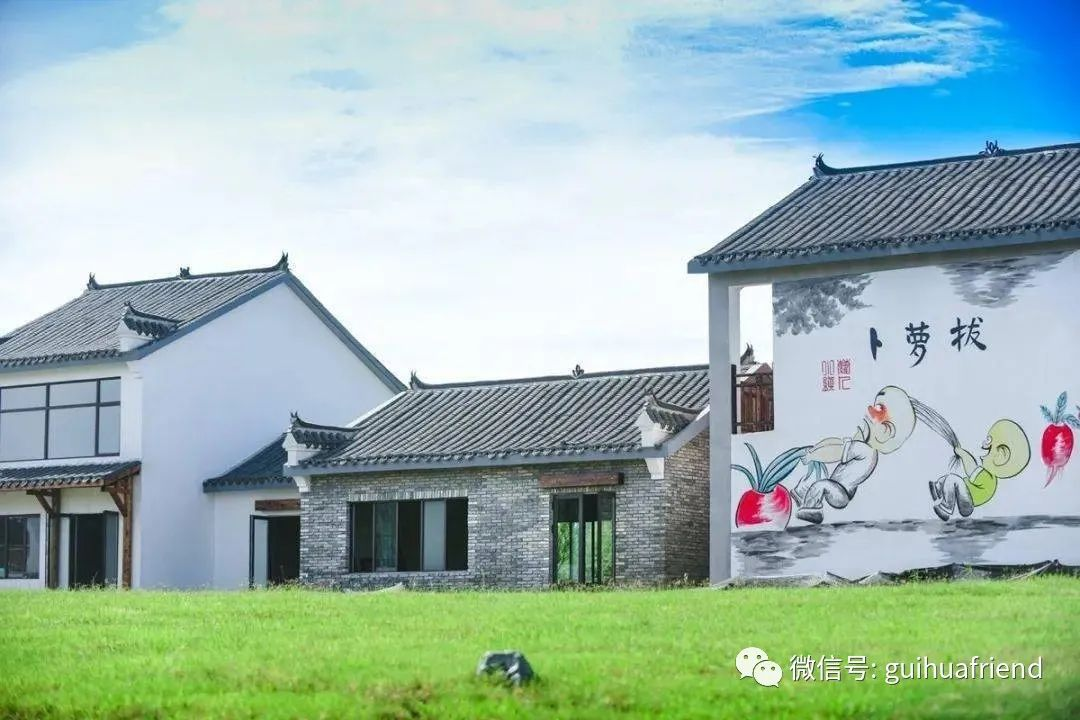
\includegraphics[width = .5\textwidth]{./ch/18.jpg}

\end{figure}



每个人都有自己的乐园,我也不例外,我的乐园不仅美丽,而且也很好玩,它就是萝卜小镇。



星期天,妈妈带我去萝卜小镇玩。萝卜小镇里长满了绿油油的小草,一眼望去真像一块碧绿的地毯。那还有一条小溪,小溪里有一群小鱼,聚在一起,像是在说悄悄话。里面有飞鸟乐园,有水上乐园,还有萌宠乐园等等好玩的地方。

我先来到飞鸟乐园。飞鸟乐园里到处都是小鸟,小鸟的羽毛,五颜六色的好看极了。最令我感兴趣的是,这里的百灵鸟。都说百灵鸟的歌声非常美妙,今天我就来听一听,果真,百灵鸟的歌声,如书上所说的一模一样,非常动听。

我们接着来到了水上乐园。水上乐园并不是有水的,因为天气的变化,水就渐渐消失了,只有小水洼,躺在那儿。那没有什么有趣的东西,但有可以让人休息的地方。

我们最后来到萌宠乐园,萌宠乐园是我最喜欢的地方,那有许许多多可爱的小动物,妈妈带我去买了些饲料,我将饲料拿去给小动物们吃。我一眼看向驴子,强烈的好奇心催促我把饲料给驴吃。我取出一根萝卜给它吃,它张开了大嘴,吓我一跳,因为驴的牙齿又大又不整齐,而且还很黄。我心想:这的饲养员能不能给驴刷个牙齿呢?真是太吓人了!

这就是我爱的乐园,它带给我无尽快乐的同时,也给我的童年增添了许多美好的回忆。





\vspace{10pt}



作者:四(3)班 龙紫怡



指导老师:徐美玲



投稿:2021年5月21日



发表:2021年5月24日


















                



\vspace{10pt}

\hline



